\documentclass[11pt]{article}


\usepackage[toc,page]{appendix}
\usepackage{amsmath, amssymb}
\usepackage{bm}% bold math
\usepackage{cancel, caption}
\usepackage{dcolumn}% Align table columns on decimal point
\usepackage{epsfig, epsf}
\usepackage{graphicx,fancyhdr,natbib,subfigure}
\usepackage{lscape, longtable}
\usepackage{hyperref,ifthen}
\usepackage{verbatim}
\usepackage{color}
\usepackage[usenames,dvipsnames]{xcolor}
\usepackage{listings}
%% http://en.wikibooks.org/wiki/LaTeX/Colors



%%%%%%%%%%%%%%%%%%%%%%%%%%%%%%%%%%%%%%%%%%%
%       define Journal abbreviations      %
%%%%%%%%%%%%%%%%%%%%%%%%%%%%%%%%%%%%%%%%%%%
\def\nat{Nat} \def\apjl{ApJ~Lett.} \def\apj{ApJ}
\def\apjs{ApJS} \def\aj{AJ} \def\mnras{MNRAS}
\def\prd{Phys.~Rev.~D} \def\prl{Phys.~Rev.~Lett.}
\def\plb{Phys.~Lett.~B} \def\jhep{JHEP} \def\nar{NewAR}
\def\npbps{NUC.~Phys.~B~Proc.~Suppl.} \def\prep{Phys.~Rep.}
\def\pasp{PASP} \def\aap{Astron.~\&~Astrophys.} \def\araa{ARA\&A}
\def\jcap{\ref@jnl{J. Cosmology Astropart. Phys.}}%
\def\physrep{Phys.~Rep.}

\newcommand{\preep}[1]{{\tt #1} }

%%%%%%%%%%%%%%%%%%%%%%%%%%%%%%%%%%%%%%%%%%%%%%%%%%%%%
%              define symbols                       %
%%%%%%%%%%%%%%%%%%%%%%%%%%%%%%%%%%%%%%%%%%%%%%%%%%%%%
\def \Mpc {~{\rm Mpc} }
\def \Om {\Omega_0}
\def \Omb {\Omega_{\rm b}}
\def \Omcdm {\Omega_{\rm CDM}}
\def \Omlam {\Omega_{\Lambda}}
\def \Omm {\Omega_{\rm m}}
\def \ho {H_0}
\def \qo {q_0}
\def \lo {\lambda_0}
\def \kms {{\rm ~km~s}^{-1}}
\def \kmsmpc {{\rm ~km~s}^{-1}~{\rm Mpc}^{-1}}
\def \hmpc{~\;h^{-1}~{\rm Mpc}} 
\def \hkpc{\;h^{-1}{\rm kpc}} 
\def \hmpcb{h^{-1}{\rm Mpc}}
\def \dif {{\rm d}}
\def \mlim {m_{\rm l}}
\def \bj {b_{\rm J}}
\def \mb {M_{\rm b_{\rm J}}}
\def \mg {M_{\rm g}}
\def \qso {_{\rm QSO}}
\def \lrg {_{\rm LRG}}
\def \gal {_{\rm gal}}
\def \xibar {\bar{\xi}}
\def \xis{\xi(s)}
\def \xisp{\xi(\sigma, \pi)}
\def \Xisig{\Xi(\sigma)}
\def \xir{\xi(r)}
\def \max {_{\rm max}}
\def \gsim { \lower .75ex \hbox{$\sim$} \llap{\raise .27ex \hbox{$>$}} }
\def \lsim { \lower .75ex \hbox{$\sim$} \llap{\raise .27ex \hbox{$<$}} }
\def \deg {^{\circ}}
%\def \sqdeg {\rm deg^{-2}}
\def \deltac {\delta_{\rm c}}
\def \mmin {M_{\rm min}}
\def \mbh  {M_{\rm BH}}
\def \mdh  {M_{\rm DH}}
\def \msun {M_{\odot}}
\def \z {_{\rm z}}
\def \edd {_{\rm Edd}}
\def \lin {_{\rm lin}}
\def \nonlin {_{\rm non-lin}}
\def \wrms {\langle w_{\rm z}^2\rangle^{1/2}}
\def \dc {\delta_{\rm c}}
\def \wp {w_{p}(\sigma)}
\def \PwrSp {\mathcal{P}(k)}
\def \DelSq {$\Delta^{2}(k)$}
\def \WMAP {{\it WMAP \,}}
\def \cobe {{\it COBE }}
\def \COBE {{\it COBE \;}}
\def \HST  {{\it HST \,\,}}
\def \Spitzer  {{\it Spitzer \,}}
\def \ATLAS {VST-AA$\Omega$ {\it ATLAS} }
\def \BEST   {{\tt best} }
\def \TARGET {{\tt target} }
\def \TQSO   {{\tt TARGET\_QSO}}
\def \HIZ    {{\tt TARGET\_HIZ}}
\def \FIRST  {{\tt TARGET\_FIRST}}
\def \zc {z_{\rm c}}
\def \zcz {z_{\rm c,0}}

\newcommand{\ltsim}{\raisebox{-0.6ex}{$\,\stackrel
        {\raisebox{-.2ex}{$\textstyle <$}}{\sim}\,$}}
\newcommand{\gtsim}{\raisebox{-0.6ex}{$\,\stackrel
        {\raisebox{-.2ex}{$\textstyle >$}}{\sim}\,$}}
\newcommand{\simlt}{\raisebox{-0.6ex}{$\,\stackrel
        {\raisebox{-.2ex}{$\textstyle <$}}{\sim}\,$}}
\newcommand{\simgt}{\raisebox{-0.6ex}{$\,\stackrel
        {\raisebox{-.2ex}{$\textstyle >$}}{\sim}\,$}}

\newcommand{\Msun}{M_\odot}
\newcommand{\Lsun}{L_\odot}
\newcommand{\lsun}{L_\odot}
\newcommand{\Mdot}{\dot M}

\newcommand{\sqdeg}{deg$^{-2}$}
\newcommand{\lya}{Ly$\alpha$\ }
%\newcommand{\lya}{Ly\,$\alpha$\ }
\newcommand{\lyaf}{Ly\,$\alpha$\ forest}
%\newcommand{\eg}{e.g.~}
%\newcommand{\etal}{et~al.~}
\newcommand{\lyb}{Ly$\beta$\ }
\newcommand{\cii}{C\,{\sc ii}\ }
\newcommand{\ciii}{C\,{\sc iii}]\ }
\newcommand{\civ}{C\,{\sc iv}\ }
\newcommand{\SiIV}{Si\,{\sc iv}\ }
\newcommand{\mgii}{Mg\,{\sc ii}\ }
\newcommand{\feii}{Fe\,{\sc ii}\ }
\newcommand{\feiii}{Fe\,{\sc iii}\ }
\newcommand{\caii}{Ca\,{\sc ii}\ }
\newcommand{\halpha}{H\,$\alpha$\ }
\newcommand{\hbeta}{H\,$\beta$\ }
\newcommand{\hgamma}{H\,$\gamma$\ }
\newcommand{\hdelta}{H\,$\delta$\ }
\newcommand{\oi}{[O\,{\sc i}]\ }
\newcommand{\oii}{[O\,{\sc ii}]\ }
\newcommand{\oiii}{[O\,{\sc iii}]\ }
\newcommand{\heii}{[He\,{\sc ii}]\ }
\newcommand{\nv}{N\,{\sc v}\ }
\newcommand{\nev}{Ne\,{\sc v}\ }
\newcommand{\neiii}{[Ne\,{\sc iii}]\ }
\newcommand{\aliii}{Al\,{\sc iii}\ }
\newcommand{\siiii}{Si\,{\sc iii}]\ }


%%%%%%%%%%%%%%%%%%%%%%%%%%%%%%%%%%%%%%%%%%%%%%%%%%%%%
%              define Listings                       %
%%%%%%%%%%%%%%%%%%%%%%%%%%%%%%%%%%%%%%%%%%%%%%%%%%%%%
\definecolor{dkgreen}{rgb}{0,0.6,0}
\definecolor{gray}{rgb}{0.5,0.5,0.5}
\definecolor{mauve}{rgb}{0.58,0,0.82}

\lstset{frame=tb,
  language=Python,
  aboveskip=3mm,
  belowskip=3mm,
  showstringspaces=false,
  columns=flexible,
  basicstyle={\small\ttfamily},
  numbers=none,
  numberstyle=\tiny\color{gray},
  keywordstyle=\color{blue},
  commentstyle=\color{dkgreen},
  stringstyle=\color{mauve},
  breaklines=true,
  breakatwhitespace=true,
  tabsize=3
}


\setlength {\textwidth}{180mm} 
\setlength {\textheight}{260mm}
\topmargin=-35.00mm
\oddsidemargin=-10.00mm
\pagestyle{empty}


\usepackage[toc,page]{appendix}
\usepackage{amsmath, amssymb}
\usepackage{bm}% bold math
\usepackage{cancel, caption}
\usepackage{dcolumn}% Align table columns on decimal point
\usepackage{epsfig, epsf}
\usepackage{graphicx,fancyhdr,natbib,subfigure}
\usepackage{lscape, longtable}
\usepackage{hyperref,ifthen}
\usepackage{verbatim}
\usepackage{color}
\usepackage[usenames,dvipsnames]{xcolor}
\usepackage{listings}
%% http://en.wikibooks.org/wiki/LaTeX/Colors



%%%%%%%%%%%%%%%%%%%%%%%%%%%%%%%%%%%%%%%%%%%
%       define Journal abbreviations      %
%%%%%%%%%%%%%%%%%%%%%%%%%%%%%%%%%%%%%%%%%%%
\def\nat{Nat} \def\apjl{ApJ~Lett.} \def\apj{ApJ}
\def\apjs{ApJS} \def\aj{AJ} \def\mnras{MNRAS}
\def\prd{Phys.~Rev.~D} \def\prl{Phys.~Rev.~Lett.}
\def\plb{Phys.~Lett.~B} \def\jhep{JHEP} \def\nar{NewAR}
\def\npbps{NUC.~Phys.~B~Proc.~Suppl.} \def\prep{Phys.~Rep.}
\def\pasp{PASP} \def\aap{Astron.~\&~Astrophys.} \def\araa{ARA\&A}
\def\jcap{\ref@jnl{J. Cosmology Astropart. Phys.}}%
\def\physrep{Phys.~Rep.}

\newcommand{\preep}[1]{{\tt #1} }

%%%%%%%%%%%%%%%%%%%%%%%%%%%%%%%%%%%%%%%%%%%%%%%%%%%%%
%              define symbols                       %
%%%%%%%%%%%%%%%%%%%%%%%%%%%%%%%%%%%%%%%%%%%%%%%%%%%%%
\def \Mpc {~{\rm Mpc} }
\def \Om {\Omega_0}
\def \Omb {\Omega_{\rm b}}
\def \Omcdm {\Omega_{\rm CDM}}
\def \Omlam {\Omega_{\Lambda}}
\def \Omm {\Omega_{\rm m}}
\def \ho {H_0}
\def \qo {q_0}
\def \lo {\lambda_0}
\def \kms {{\rm ~km~s}^{-1}}
\def \kmsmpc {{\rm ~km~s}^{-1}~{\rm Mpc}^{-1}}
\def \hmpc{~\;h^{-1}~{\rm Mpc}} 
\def \hkpc{\;h^{-1}{\rm kpc}} 
\def \hmpcb{h^{-1}{\rm Mpc}}
\def \dif {{\rm d}}
\def \mlim {m_{\rm l}}
\def \bj {b_{\rm J}}
\def \mb {M_{\rm b_{\rm J}}}
\def \mg {M_{\rm g}}
\def \qso {_{\rm QSO}}
\def \lrg {_{\rm LRG}}
\def \gal {_{\rm gal}}
\def \xibar {\bar{\xi}}
\def \xis{\xi(s)}
\def \xisp{\xi(\sigma, \pi)}
\def \Xisig{\Xi(\sigma)}
\def \xir{\xi(r)}
\def \max {_{\rm max}}
\def \gsim { \lower .75ex \hbox{$\sim$} \llap{\raise .27ex \hbox{$>$}} }
\def \lsim { \lower .75ex \hbox{$\sim$} \llap{\raise .27ex \hbox{$<$}} }
\def \deg {^{\circ}}
%\def \sqdeg {\rm deg^{-2}}
\def \deltac {\delta_{\rm c}}
\def \mmin {M_{\rm min}}
\def \mbh  {M_{\rm BH}}
\def \mdh  {M_{\rm DH}}
\def \msun {M_{\odot}}
\def \z {_{\rm z}}
\def \edd {_{\rm Edd}}
\def \lin {_{\rm lin}}
\def \nonlin {_{\rm non-lin}}
\def \wrms {\langle w_{\rm z}^2\rangle^{1/2}}
\def \dc {\delta_{\rm c}}
\def \wp {w_{p}(\sigma)}
\def \PwrSp {\mathcal{P}(k)}
\def \DelSq {$\Delta^{2}(k)$}
\def \WMAP {{\it WMAP \,}}
\def \cobe {{\it COBE }}
\def \COBE {{\it COBE \;}}
\def \HST  {{\it HST \,\,}}
\def \Spitzer  {{\it Spitzer \,}}
\def \ATLAS {VST-AA$\Omega$ {\it ATLAS} }
\def \BEST   {{\tt best} }
\def \TARGET {{\tt target} }
\def \TQSO   {{\tt TARGET\_QSO}}
\def \HIZ    {{\tt TARGET\_HIZ}}
\def \FIRST  {{\tt TARGET\_FIRST}}
\def \zc {z_{\rm c}}
\def \zcz {z_{\rm c,0}}

\newcommand{\ltsim}{\raisebox{-0.6ex}{$\,\stackrel
        {\raisebox{-.2ex}{$\textstyle <$}}{\sim}\,$}}
\newcommand{\gtsim}{\raisebox{-0.6ex}{$\,\stackrel
        {\raisebox{-.2ex}{$\textstyle >$}}{\sim}\,$}}
\newcommand{\simlt}{\raisebox{-0.6ex}{$\,\stackrel
        {\raisebox{-.2ex}{$\textstyle <$}}{\sim}\,$}}
\newcommand{\simgt}{\raisebox{-0.6ex}{$\,\stackrel
        {\raisebox{-.2ex}{$\textstyle >$}}{\sim}\,$}}

\newcommand{\Msun}{M_\odot}
\newcommand{\Lsun}{L_\odot}
\newcommand{\lsun}{L_\odot}
\newcommand{\Mdot}{\dot M}

\newcommand{\sqdeg}{deg$^{-2}$}
\newcommand{\lya}{Ly$\alpha$\ }
%\newcommand{\lya}{Ly\,$\alpha$\ }
\newcommand{\lyaf}{Ly\,$\alpha$\ forest}
%\newcommand{\eg}{e.g.~}
%\newcommand{\etal}{et~al.~}
\newcommand{\lyb}{Ly$\beta$\ }
\newcommand{\cii}{C\,{\sc ii}\ }
\newcommand{\ciii}{C\,{\sc iii}]\ }
\newcommand{\civ}{C\,{\sc iv}\ }
\newcommand{\SiIV}{Si\,{\sc iv}\ }
\newcommand{\mgii}{Mg\,{\sc ii}\ }
\newcommand{\feii}{Fe\,{\sc ii}\ }
\newcommand{\feiii}{Fe\,{\sc iii}\ }
\newcommand{\caii}{Ca\,{\sc ii}\ }
\newcommand{\halpha}{H\,$\alpha$\ }
\newcommand{\hbeta}{H\,$\beta$\ }
\newcommand{\hgamma}{H\,$\gamma$\ }
\newcommand{\hdelta}{H\,$\delta$\ }
\newcommand{\oi}{[O\,{\sc i}]\ }
\newcommand{\oii}{[O\,{\sc ii}]\ }
\newcommand{\oiii}{[O\,{\sc iii}]\ }
\newcommand{\heii}{[He\,{\sc ii}]\ }
\newcommand{\nv}{N\,{\sc v}\ }
\newcommand{\nev}{Ne\,{\sc v}\ }
\newcommand{\neiii}{[Ne\,{\sc iii}]\ }
\newcommand{\aliii}{Al\,{\sc iii}\ }
\newcommand{\siiii}{Si\,{\sc iii}]\ }


%%%%%%%%%%%%%%%%%%%%%%%%%%%%%%%%%%%%%%%%%%%%%%%%%%%%%
%              define Listings                       %
%%%%%%%%%%%%%%%%%%%%%%%%%%%%%%%%%%%%%%%%%%%%%%%%%%%%%
\definecolor{dkgreen}{rgb}{0,0.6,0}
\definecolor{gray}{rgb}{0.5,0.5,0.5}
\definecolor{mauve}{rgb}{0.58,0,0.82}

\lstset{frame=tb,
  language=Python,
  aboveskip=3mm,
  belowskip=3mm,
  showstringspaces=false,
  columns=flexible,
  basicstyle={\small\ttfamily},
  numbers=none,
  numberstyle=\tiny\color{gray},
  keywordstyle=\color{blue},
  commentstyle=\color{dkgreen},
  stringstyle=\color{mauve},
  breaklines=true,
  breakatwhitespace=true,
  tabsize=3
}

\begin{document}

\title{Accreting BH Timescales}
\author{NPR, Andy Lawrence, Chelsea MacLeod, Alastair Bruce}
\date{\today}
\maketitle


\begin{abstract}
A list of Accreting BH timescales, and how they scale 
with e.g. $M_{\rm BH}$. 
(See also ``General\_Physical\_terms'' and ``Xray Terminology).
\end{abstract}


%Section heading
\section{Accreting BH timescales}
General notes: a 1$\times10^{8}$ M$_{\odot}$ has a Schwarzschild Radius of $R_{\rm
Schwarz}=2.954 \times10^{8}$ km. \\
And 1 AU is 1.496$\times10^{8}$ km.  \\ 
Light travel time across this $R_{S}$ is 984.77 seconds.
%% https://www.omnicalculator.com/physics/schwarzschild-radius 


\subsection{Light crossing}
The light crossing timescale; variations in light output cannot occur on timescales less than this.

\begin{table}
  \begin{center}
    % \begin{tabular}{l ccc c } 
    \begin{tabular}{l l l l l l} 
      \hline
      \hline 
      Timescale         &     Equation    &  Ref  \\
      \hline  
       &&& \\
       light crossing  &  {\boldmath $t_{\rm lt} = R/c$}       &  \multirow{4}{*}{FKR2002, Eqn~(7.4) }      \\
                               &   $ \geq 2GM /c^{3}$                                 &  \\
                               &  $= 0.98\times10^{-5} (M/M_{\odot})$ secs   &  \\
                                &   = 980 seconds (for the 1e8 $M_{\odot}$ given above ;-) & \\ 
        &&& \\
         \hline
         \hline 
       \end{tabular}
      \caption{Light Crossing timescale; variations in light output cannot occur on timescales less than this.}
      \label{tab:lightcrossing}
    \end{center}
\end{table}


\subsection{Dynamical}
The shortest characteristic timescale of the disc is the dynamical timescale. 

\begin{table}
  \begin{center}
    % \begin{tabular}{l ccc c } 
    \begin{tabular}{l l l l l l} 
      \hline
      \hline 
      Timescale   & Equation    &  Ref  \\
      \hline  
       &&& \\
       dynamical  & $t_{\rm dyn} = \sqrt{R^{3}/c}$ &     \\
                          &  $\sim R/v_{\phi}$           &  \multirow{3}{*}{FKR2002, Eqn~(5.63) }  \\
                          & $t_{\phi} \sim \Omega_{K}^{-1}$                                             &  \\
        &&& \\
         \hline
         \hline 
       \end{tabular}
      \caption{The shortest characteristic timescale of the disc is the dynamical timescale.}
      \label{tab:lightcrossing}
    \end{center}
\end{table}


\subsection{Sound}
The general sound crossing timescale. 
Sound speed, given as:
\begin{equation}
     c_{s} =  \left (\frac{d P}{d \rho} \right)^{1/2}_{0}.
\end{equation}. 
$\gamma = 5/3$ is adiabatic, while $\gamma = 1$ is isothermal.
with (from e.g. FKR2002) both $c_{s}^{\rm ad}$ and $c_{s}^{\rm iso}$
the order of the mean thermal speed of the ions of the gas,
\begin{equation}
c_{s} \approx 10 (T/10^{4} K)^{1/2} km s^{-1}
\end{equation}

\begin{table}
  \begin{center}
    % \begin{tabular}{l ccc c } 
    \begin{tabular}{l l l l l l} 
      \hline
      \hline 
      Timescale           &                       Equation    &  Ref  \\
      \hline  
       &&& \\
       Sound  &  $t_{\rm snd} = R/c_{\rm s}$                                                 &      \\
        &&& \\
         \hline
         \hline 
       \end{tabular}
      \caption{Light Crossing timescale; large variations in light output cannot occur on timescales less than this.}
      \label{tab:lightcrossing}
    \end{center}
\end{table}

\subsection{Thermal}
From e.g. FKR2002, the {\it thermal timescale:}
\begin{equation}
t_{th} = \frac{\rm heat \; content \; per \; unit \; disc \; area}{\rm dissipation \;  rate \; per \; unit \; disc \; area}.
\end{equation}
i.e. a timescale for an ``energy spike'' to dissipate within disc. 

\begin{table}
  \begin{center}
    % \begin{tabular}{l ccc c } 
    \begin{tabular}{l l l l l l} 
      \hline
      \hline 
      Timescale           &                       Equation    &  Ref  \\
      \hline  
       &&& \\
       Thermal  &     $t_{\rm th} = \mathcal{M} / t_{\rm visc}$                                                 &  \multirow{3}{*}{FKR2002}      \\
                  &                                   &  \\
                  &       &  \\
        &&& \\
         \hline
         \hline 
       \end{tabular}
      \caption{Time for an ``energy spike'' to dissipate within the disc.}
      \label{tab:lightcrossing}
    \end{center}
\end{table}
where $\mathcal{M}$ is Mach number,  $v/c_{s}$. 


\subsection{Viscous}
\begin{table}
  \begin{center}
    % \begin{tabular}{l ccc c } 
    \begin{tabular}{l l l l l l} 
      \hline
      \hline 
      Timescale           &                       Equation    &  Ref  \\
      \hline  
       &&& \\
       Viscous  &     $t_{\rm visc} = R^{2}/\nu$                                                 &  \multirow{3}{*}{FKR2002 }      \\
                  &     &  \\
              &   &  \\
        &&& \\
         \hline
         \hline 
       \end{tabular}
      \caption{where $\nu$ is {\it kinematic viscosity}. This is the ``diffusion through disc'' timescale from viscous torques.}
      \label{tab:lightcrossing}
    \end{center}
\end{table}



%\begin{landscape}
\begin{figure}
  \centering
  %% trim=l b r t 
  % \includegraphics[width=8.00cm, height=7.50cm, trim=0.0cm 0.0cm 0.0cm 0.0cm, clip] {J110057_CRTS_lightcurve_v0pnt1.png}
%  \includegraphics[width=16.00cm, height=10.00cm, trim=0.0cm 0.0cm 0.0cm 0.0cm, clip]
  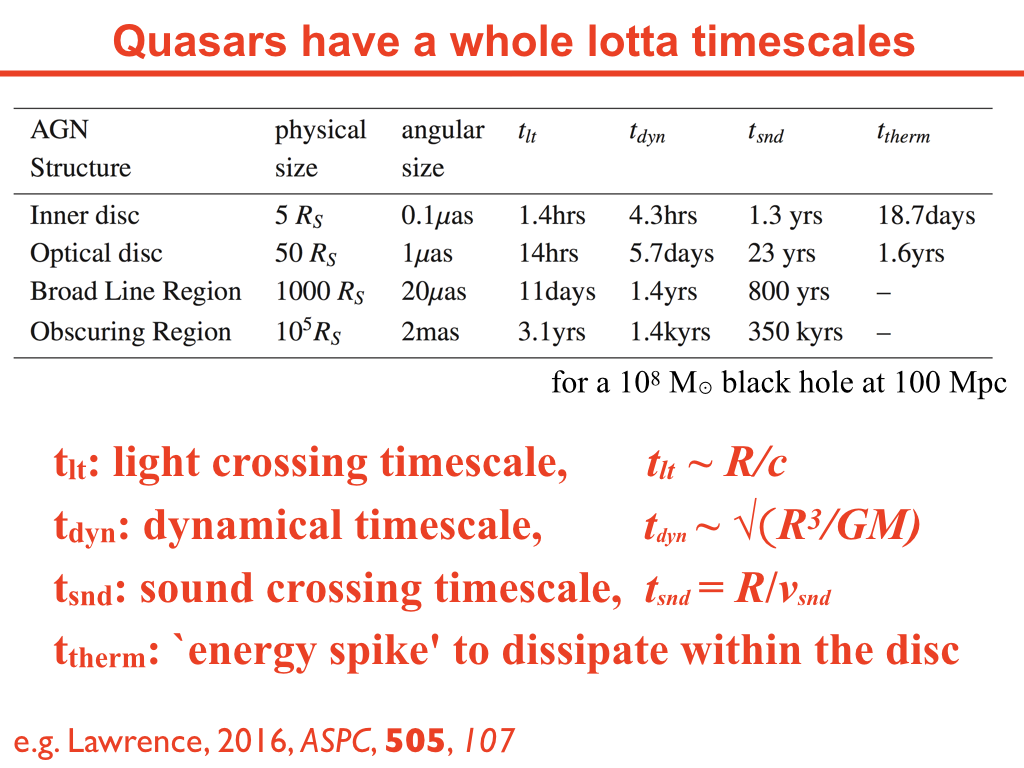
\includegraphics[width=18.00cm, height=14.00cm]{Lawrence_2016plus.png}
  \caption[]{} 
  \label{}
\end{figure}
%\end{landscape}


%\begin{landscape}
\begin{table}
  \caption{Timescales and how the scale with $M$, $R$, $T$ etc.}
  \label{tab:the_lines}
  \begin{center}
    \begin{tabular}{lr} 
      \hline
      \hline
      Name & Scaling \\ 
      \hline
      Viscous & $M^{\alpha}$ \\
     \hline
      \hline
   \end{tabular}
  \end{center}
\end{table}
%\end{landscape}

\citet{Croom2004}
\noindent




\newpage
\section{Time Scales}
From Lawrence (2016) http://adsabs.harvard.edu/abs/2016ASPC..505..107L :: \\
All Type I AGN - those where we can see the strong blue continuum and
broad emission lines - are variable.\footnote{For simplicity, I am
only going to talk about the UVOIR spectral region, ignoring X-rays.}
This is important because variability can provide indirect information
on size scales that are otherwise unmeasurable. Suppose, for
illustration, we take an AGN at a distance of 100 Mpc, and we assume
that it contains a black hole of mass $10^8$ M$_\odot$. The Table
below shows the angular scale of well known AGN structures, in units
of the Schwarzschild radius $R_S=2GM/c^2$. The accretion disc, Broad
Line Region (BLR) and the geometrically thick obscuring region
sometimes known as the ``torus'' are all unresolvable by direct means,
although as we will describe later, may be mappable by microlensing
transits.

If the accretion disc is in a stable steady state, we might expect it
to evolve gradually on the inward drift timescale set by viscosity,
which is of the order 10,000 years (see
e.g. \citet{Netzer2013}). However, instabilities of various kinds
could give us much faster changes. The {\em light crossing timescale}
$t_{lt}=R/c$, is the shortest timescale that we could possibly see, if
for example one region has variations locked to those of another
region by radiation heating or reflection. This is of the order hours,
days, and years for disc, BLR, and torus respectively. The {\em
dynamical timescale}, $t_{dyn}=\sqrt{R^3/GM}$, is the shortest
timescale on which we are likely to see physical changes in a region,
and is of the order of days, years, and thousands of years for disc,
BLR, and torus respectively. (Free-fall time is roughly the same and
orbital timescale is $2\pi$ times longer.) More realistically,
perturbations may transmit across a region on the sound crossing
timescale $t_{snd}= R/ v_{snd}$. This is somewhat model dependent but
is of the order of years for the accretion disc. Note what I mean here
is the global time to cross the whole region. Local hot spots could
grow on the timescale it takes sound to cross the vertical height of
the disc, which could be 1--3 orders of magnitude faster. Somewhat
related is the ``thermal'' timescale $t_{therm}$ which is roughly the
time it takes for for energy to dissipate within the disc, i.e. it is
a kind of response timescale to a spike of energy input. This is model
dependent of course, but some standard formulae are given in
\citet{Collier2001a} and \citet{Kelly2009}. It is of the order of days
for the inner disc and years for the optical disc.  The analogous
``response'' timescale for the BLR and for the obscuring region is
actually the light-crossing time - the local response time to a change
in photo-ionisation or heating is very short, but what we see is
smeared out by the range of light travel delays.

\begin{table}[!ht]
\begin{center}
%\caption{AGN timescales}
\smallskip
{\small
\begin{tabular}{lllllll}  % l = left, c = centered

\hline
\noalign{\smallskip}
AGN & physical & angular & $t_{lt}$ & $t_{dyn}$ & $t_{snd}$ & $t_{therm}$ \\
\noalign{\smallskip}
Structure & size & size & &  &  & \\
\noalign{\smallskip}
\hline

\noalign{\smallskip}
Inner disc & 5 $R_S$ & 0.1$\mu$as & 1.4hrs & 4.3hrs & 1.3 yrs & 18.7days \\
\noalign{\smallskip}
Optical disc & 50 $R_S$ & 1$\mu$as & 14hrs & 5.7days & 23 yrs & 1.6yrs \\
\noalign{\smallskip}
Broad Line Region & 1000 $R_S$ & 20$\mu$as & 11days & 1.4yrs & 800 yrs & -- \\
\noalign{\smallskip}
Obscuring Region & $10^5 R_S$ & 2mas & 3.1yrs & 1.4kyrs & 350 kyrs & --  \\

\noalign{\smallskip}
\hline  
\end{tabular}
}
\end{center}
\end{table}

Are these timescales relevant to what we actually see? The UV continuum changes on timescales of weeks\footnote{Here I am assuming an Seyfert-like object appropriate to our $10^8 M_\odot$ example.}, with an RMS of around $\pm 30\%$, which means trough-to-peak changes of up to a factor of two are not unusual. The variations in the optical continuum, BLR, and IR seem to track these variations with roughly the light-travel time delays suggested in the Table, together with a similar amount of smearing (see recent examples in \citet{Edelson2015}, \cite{Grier2012}, and  \citet{Koshida2014}). This strongly suggests that almost all the changes we see on the relevant timescales represent reprocessed emission driven by changes in the very central regions. The conventional explanation for many years has been that the driving power is from the X-ray source (e.g \citet{McHardy2014}), but in many cases this does not work in either energy budget or correlation terms (see \citet{Lawrence2012} and references therein). A good alternative for the driving power is the (unseen) EUV peak of the very inner accretion disc.

The amplitude we see in the optical continuum on these $\sim$week timescales (around 3\%  RMS) is much smaller than that seen in the UV variations, which suggests that a very blue variable component mixes with an unchanging, or slower changing, redder component. \citet{Lawrence2012} argues that this variable reprocessor is a system of dense inner clouds surrounding the disc, rather than the disc itself.

The variations seen in the UV, which the optical and BLR emission track, seem to follow a red-noise or random-walk like pattern, increasing in amplitude to longer timescales, flattening at a characteristic timescale of the order tens of days. This timescale depends on the mass of the black hole (Collier and Peterson 2001). This characteristic timescale seems to match the thermal timescale of the inner disc, suggesting that variability is driven by some unknown stochastic process, filtered by the physical response of the disc \citep{Kelly2009, Kelly2011}.

Note that the changes we see in broad emission lines are also of the order weeks, tracking the changes in the UV photo-ionising source. This is much shorter than the dynamical timescale of the BLR, and means we are not seeing structural changes in this region. In the popular "local optimally emitting cloud (LOC)" models we will be lighting up different pre-existing clouds at different distances as the UV goes up and down \citep{Peterson2006,Goad2014}, which is why the amplitude of line variations (the ``responsivity'') varies with line species - Ly $\alpha$ has a large amplitude and Mg II hardly varies at all (e.g. \citet{Cackett2015}). However, it is possible that on longer timescales we {\em will} see BLR structural changes - a point we will return to in section 5.3.


\medskip \medskip
\noindent
From Aneta Siemiginowska's talk::\\
Light crossing time at 100 $r_{\rm s}$:
\begin{equation}
    t_{\rm lc} = 1.1 \,  M_{8} \, R_{100 r_{S}}  \; {\rm days}
\end{equation}

\noindent
Orbital::
\begin{equation}
  t_{\rm orb} = 104 \, M_{8} \,  (R_{100r_{S}})^{3/2} \;  {\rm days}
\end{equation}

\noindent
Thermal (note the viscosity dependence)
\begin{equation}
  t_{\rm th} = 4.6 \, (\alpha_{0.01})^{-1} \, M_{8}\, (R_{100r_{S}} )^{3/2}  \; {\rm years}
\end{equation}
$r_{s} = 2 \,  GM_{\rm bh}/c^{2}$ \\ 
$R_{100r_{S}} = \, R / 100 r_{S}$  \\
$M_{8} = \,  M_{\rm bh} /10^{8} M_{\odot}$.

\medskip
\noindent
Note:: 
\begin{equation}
  \Rightarrow t_{\rm th} \sim (h/r)^{2} t_{\rm visc}
\end{equation}


\newpage


\begin{table}
  \begin{center}
    % \begin{tabular}{l ccc c } 
    \begin{tabular}{l l l l l l} 
      \hline
      \hline 
      Timescale     &          & Equation                                                                                                         & Baseline& Range& Ref \\
      \hline  
      \hline 
      Apocenter            & apo     & $v_{\rm radial}/g$                                                                                     &            &             & Elvis17\\
                                  &             &    $75 v_{1000}. R_{1000} 2 M8$ d                                                             & & & Elvis17\\ 
      Cloud crossing    &  cc         &    & & & \\
      Cloud crushing    & ccr       &     & & & \\
      Cooling time       & cool      &    & & & Elvis17\\
%   Dynamical            & dyn       & $(R^3/GM)^{1/2} = P_{\rm orb}/2\pi = 1.4 \; R_{1000}^{3/2} \; M_{8} \; {\rm yr}$          &   & & \\
      Dynamical            & dyn    & $(R^3/GM)^{1/2}$                                                                                                 &   & & Elvis17\\
                                   &          & $P_{\rm orb}/2\pi$                                                                                                 &   & & Elvis17\\
                                   &           & $1.4 \; R_{1000}^{3/2} \; M_{8} \; {\rm yr}$                                                             &   & & Elvis17\\
       %     Escape         &  esc   &  $v_{\rm esc} / g = (v_{\rm esc} / v_{\rm Kep}) . \tau_{\rm dyn} = 1.4 \tau_{\rm dyn} \; s $  & & & \\
      Escape                 &  esc  &  $v_{\rm esc} / g$                                                                                                         & & & Elvis17\\
                                  &          & $(v_{\rm esc} / v_{\rm Kep}) . \tau_{\rm dyn} $       & & & \\
                                  &            & $1.4 \tau_{\rm dyn} \; s $                                 & & & \\
      Light Crossing     & lc           &   $1.1 \,  M_{8} \, R_{100 r_{S}}  \; {\rm days}$   &   & & SiemUSVI17\\ 
                                  &               &  $ R / c$                                                            &   & & Lawrence16 \\ 
      Orbital                 &  orb    &     $104 \, M_{8} \,  (R_{100r_{S}})^{3/2} \;  {\rm days}$ & & & SiemUSVI17\\ 
      Sound crossing    &  sound  &     $ R / v_{\rm snd} $ & & & \\     
       Thermal               &   th     &    $4.6 \, (\alpha_{0.01})^{-1} \, M_{8}\, (R_{100r_{S}} )^{3/2}  \; {\rm years}$  & & & SiemUSVI17\\ 
                                   &           &   $\sim (h/r)^{2} t_{\rm visc}$                        & & & SiemUSVI17\\ 
      Viscous                 & visc  & 12.6 yr $L_{\rm E}^{-3/10} \, M_8^{6/5} R_{30}^{5/4} \alpha_{0.1}^{-4.5} \mu_{0.1}^{3/10}$  & & & Lawrence12 \\
      X-ray                    & X             &    & & & \\
         \hline
         \hline 
       \end{tabular}
      \caption{SiemUSVI17 is Aneta Siemiginowska's talk in the USVI Extreme AGN 2017 meeting.}
%                    \href{https://github.com/d80b2t}{\tt github.com/d80b2t}
      \label{SiemUSVI17}
    \end{center}
\end{table}

\noindent
Where:\\
$\alpha$ is the viscosity parameter; \\
$cs = (\gamma k_{\rm B} T/\mu m_{\rm H}^{1/2}) = 150 T_{6}^{1/2} km s^{-1}$ \\
$g$ is the local acceleration due to gravity, GM/R2; \\
$G$ is the gravitational constant; \\
$k_{\rm B}$ is Boltzmann’s constant = $1.38 \times10^{-16}$ erg K$^{-1}$;\\
$L/LEdd$ is the Eddington ratio; \\
$Lbol,44$ is the ultraviolet bolometric luminosity in units of 1044 erg s-1;\\
$\mathcal{M}$  is the Mach number; \\
$M$ is the mass of the black hole in solar masses;\\
$M_{8}$ is $M$ in units of 10$^{8}$ solar masses;\\
$m_{\rm H}$ is the mass of the hydrogen atom = $1.67\times10^{-24}$ g;\\
$\mu$ is the efficiency parameter; \\
P$_{\rm orb}$ is the orbital period in s;\\
$R$ is the distance from the central black hole in cm;\\
$R_{\rm 1000}$ = is $R$ in units of 1000 Schwarzschild radii, $rg = 2GM/c2$; \\
$ri,13$ is ri the initial radius of a condensing cloud in units of 1013 cm;\\
$rc$ is the radius of the condensed cloud, = ri $\chi$1/3, for a density ratio of $\chi$; i.e. 0.22 $\chi$ for a density ratio of 100; (double check this!!!)\\
$T_{\rm i,6}$ is the initial temperature of the wind in units of 106 K; \\
$v_{\rm 1000}$ = initial radial WA velocity in units of 1000 km s-1; \\
$v_{\rm esc}$ = (2GM/R)1/2 is the escape velocity from radius  %R = 9500 R1000 km s$^{-1}$ = $\sqrt$2$\times$6700 -  1000 km s$^{-1}$; \\
$Z/Z$ is gas metallicity relative to solar (section 2.1); \\
$\Lambda$ is the cooling coefficient (erg s-1 cm3) ; \\
$\Lambda_{\rm b} (T)$ is the cooling coefficient for bremsstrahlung; \\
$\Lambda (T) /\Lambda_{\rm b}$  is the factor increase in the cooling
coefficient in a thermal plasma due to line cooling over
bremsstrahlung at solar metallicity, which has values of $\sim$35 for 
T =105 - 106 K, ~100forT=104.5 K, and peaks at$\sim$500 for $T=10^{5-5.5}$ K;\\
$\gamma$ is the ideal gas adiabatic index $= 5/3$; \\
$\mu$ is the mean molecular weight of the gas ($\sim$0.6); and\\
$\chi$ is the ratio of the cloud density to the ambient medium density.





\bibliographystyle{mn2e}
\bibliography{/cos_pc19a_npr/LaTeX/tester_mnras}

\end{document}

